% Sample tex file for usage of iidef.sty
% Homework template for Inference and Information
% UPDATE: October 12, 2017 by Xiangxiang
% UPDATE: 22/03/2018 by zhaofeng-shu33
\documentclass[a4paper]{article}
\usepackage[T1]{fontenc}
\usepackage{amsmath, amssymb, amsthm}
% amsmath: equation*, amssymb: mathbb, amsthm: proof
\usepackage{moreenum}
\usepackage{mathtools}
\usepackage{url}
\usepackage{graphicx}
\usepackage{subcaption}
\usepackage{booktabs} % toprule
\usepackage[mathcal]{eucal}
\usepackage{dsfont}

\usepackage[numbered,framed]{matlab-prettifier}
\lstset{
  style              = Matlab-editor,
  captionpos         =b,
  basicstyle         = \mlttfamily,
  escapechar         = ",
  mlshowsectionrules = true,
}

\usepackage[thehwcnt = 6]{iidef}
\thecourseinstitute{Tsinghua-Berkeley Shenzhen Institute}
\thecoursename{Information Inference}
\theterm{Fall 2017}
\hwname{Coursework}
\begin{document}
\courseheader
\name{YOUR NAME}
\rule{\textwidth}{1pt}
\begin{itemize}
\item {\bf Acknowledgments: \/} 
  This template takes some materials from course CSE 547/Stat 548, University of Washington: \small{\url{https://courses.cs.washington.edu/courses/cse547/17sp/index.html}}.

  If you refer to other materials in your homework, please list here.
\item {\bf Collaborators: \/}
  I finish this template by myself. If you finish your homework all by yourself, make a similar statement. If you get help from others in finishing your homework, state like this:
  \begin{itemize}
  \item 1.2 (b) was solved with the help from \underline{\hspace{3em}}.
  \item Discussion with \underline{\hspace{3em}} helped me finishing 1.3.
  \end{itemize}
\end{itemize}
\rule{\textwidth}{1pt}

\vspace{2em}

You may use \texttt{enumerate} to generate answers for each question:

\begin{enumerate}
  \setlength{\itemsep}{3\parskip}

  \item Type of commonly used notations. Use another \texttt{enumerate} to start generate answers for sub-questions:
    \begin{enumerate}
    \item Use \verb|$ $| to get an inline equation: $\Prob(A) = \E[\1_A(\omega)]$.
    \item Use \texttt{equation} to have equation in display math mode:
      \begin{equation}
        \frac{a + b}{2} \geq \sqrt{ab}
        \label{eq:1}
      \end{equation}
      
    \item Use \verb|\eqref| to get reference for equations: \eqref{eq:1} holds when $a\geq 0, b\geq 0$.
      
    \item Now we would introduce some commonly used notations:
      \begin{enumerate}
      \item Use \verb|\mathbb{P}, \mathbb{R}, \mathbb{E}| to type $\mathbb{P}, \mathbb{R}, \mathbb{E}$.
      \item Use \verb|\mathcal{A}, \mathcal{X}, \mathcal{Y}, \mathcal{N}| to type $\mathcal{A}, \mathcal{X}, \mathcal{Y}, \mathcal{N}$.
      \item Use \verb|\underline{x}, \underline{y}| to type vectors $\underline{x}, \underline{y}$.
      \item Use \verb|\mathsf{x}, \mathsf{y}, \mathsf{z}| to type random variables $\rvx, \rvy, \rvz$. For simplicity, I have defined several macros so you could simply type \verb|\rvx, \rvy, \rvz|. Don't forget \verb|$ $|!
      \item Thanks to these macros, we could have $\reals, \E[\rvx], \Var(\rvy), \Prob(A), \independent, \1$ by typing \verb|\reals, \E[\rvx], \Var(\rvy), \Prob(A),\independent,| \verb|\1|.
      \item Now you can use \verb|\ux, \uy, \uz| to type vectors $\ux, \uy, \uz$, and use \verb|\urvx, \urvy, \urvz| to type random vectors $\urvx, \urvy, \urvz$.   
      \item Remember that $P_{\rvx|\rvy}(x|y) \defas \Prob(\rvx = x|\rvy = y)$.
        \begin{enumerate}
        \item Writing $\Prob(x)$ is wrong. $\Prob$ should only operate on events.
        \item $\rvx$ is a random variable, while $x$ is a real number.
        \end{enumerate}
        
      \end{enumerate}
    \item You may find \url{https://en.wikibooks.org/wiki/LaTeX} useful.
    \item Writing \LaTeX\ online may be easier for beginners:
        \begin{enumerate}
        \item ShareLaTeX: \url{https://www.sharelatex.com/}.
        \item Overleaf: \url{https://www.overleaf.com/}.
        \end{enumerate}
    \end{enumerate}
  \item You may need aligned equations for your homework, here are several examples:
    
    Total propability rule:
  \begin{equation*}
    \begin{aligned}
      \Prob(\rvx = x)
      &= \sum_{y \in \mathcal{Y}} \Prob(\rvx = x, \rvy = y)\\
      &= \sum_{y \in \mathcal{Y}} \Prob(\rvx = x| \rvy = y) \Prob(\rvy = y),\\
    \end{aligned}
  \end{equation*}
  or
  \begin{equation*}
    \begin{aligned}
      &\quad~  P_{\rvx}(x)\\
      &= \sum_{y \in \mathcal{Y}} P_{\rvx\rvy}(x,y)\\
      &= \sum_{y \in \mathcal{Y}} P_{\rvx|\rvy}(x|y)P_{\rvy}(y).\\
    \end{aligned}
  \end{equation*}
  Indicator function:
  \begin{equation*}
    \1_A(\omega)=
    \left\{
    \begin{aligned}
      1, &\quad\text{if}~ \omega \in A,\\
      0, &\quad\text{if}~ \omega \notin A.
    \end{aligned}
    \right.
  \end{equation*}

  \item You may need to add figure and source codes in your homework. Figure \ref{fig:1} is an example that compares the empirical distribution (histogram) and probability density function of the Gaussian random variable.
    \begin{figure}[htbp]
      \centering
      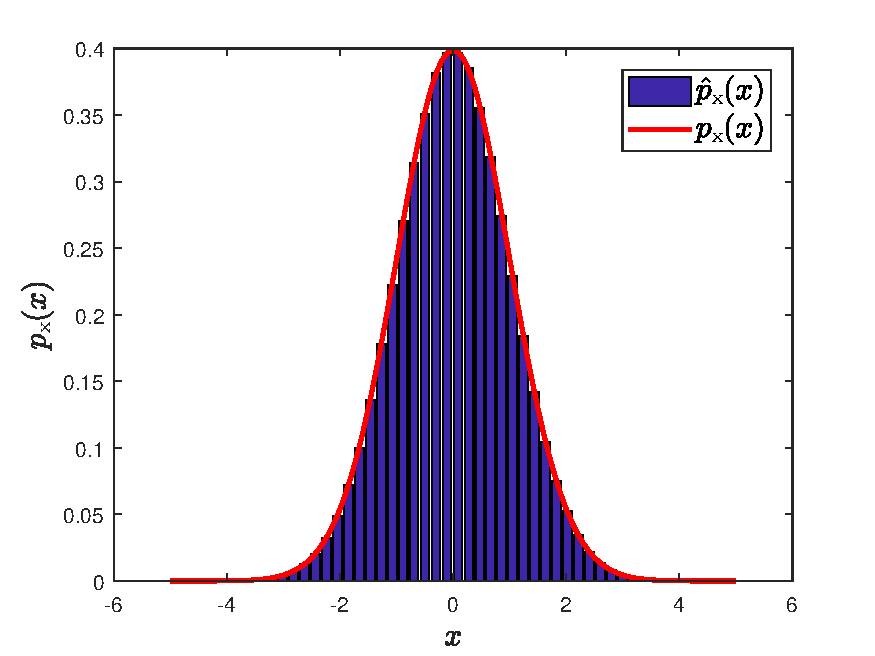
\includegraphics[width = 0.8\textwidth]{pdf_normal.pdf}
      \caption{Gaussian PDF and histogram of samples}
      \label{fig:1}
    \end{figure}

  The source code to plot Figure \ref{fig:1} could be found in Appendix \ref{sec:a:code}. Here are the core codes:
  \lstinputlisting[firstline=4,lastline=4, firstnumber=4]{matlabscript.m}
  \lstinputlisting[firstline=6,lastline=7, firstnumber=6]{matlabscript.m}
  To understand line 6, note that if we have $n$ samples of $\rvx$ denoted by $x^{(i)}, i = 1, 2, \cdots, n$, then the probability density function $p_{\rvx}$ could be estimated as
  \begin{equation*}
    \begin{aligned}
      p_{\rvx}(x_0) &= \left.\frac{\mathrm{d}}{\mathrm{d}x} \Prob(\rvx \leq x) \right|_{x = x_0} \\
      &\approx \frac{\Prob(x_0 - \Delta x < \rvx \leq x_0)}{\Delta x}\\
      &\approx \frac{1}{n\Delta x} \sum_{i = 1}^n \1_{x^{(i)} \in (x_0 - \Delta x, x_0]}.
    \end{aligned}    
  \end{equation*}
  
\item An example of hypothesis testing:
  \begin{equation*}
   \log \frac{\Prob(\rvH = H_1|\rvy = y)}{\Prob(\rvH = H_0|\rvy = y)} 
   \mathop{\gtreqless}_{\hat{\rvH} = H_0}^{\hat{\rvH} = H_1} \gamma
  \end{equation*}
  
  \end{enumerate}

  
  \newpage
  
  \appendix
  \section{Source code}
  \label{sec:a:code}
  % \lstlistoflistings
  Source code for plotting Figure \ref{fig:1} is shown as follows.
  \lstinputlisting[caption=FigurePlot]{matlabscript.m}
  
\end{document}
%%% Local Variables:
%%% mode: latex
%%% TeX-master: t
%%% End:
